\chapter{History and recent advancements}
\label{kap:kap1}

The amount of information and data grows exponentially over years. In order to store and work with this data, we use different data structures. These data structures do not only represent the data but also enable us to make certain operations over them. There is a significant effort in not only speeding up these structures but also making them smaller in size so that they can be managed in memory and not on a secondary data storage such as a disk that is often orders of magnitude times slower. The key factor is to find the right balance between the speed of common operations and the amount of information that we need to store. These data structures often find usage in bioinformatics and compression algorithms.

\section{Space-efficient data structures}

When we measure how space-efficient the data structure is, we often measure this in size of additional information that we store alongside the original data. Most of the time, with the complexity of operations that our data structure supports, the amount of helper data stored alongside the original data also increases. However, the original data can be also compressed to further increase the space-efficiency. To remove ambiguity, it is common to measure the size of the original data in the information-theoretical optimal number of bits used to store the original data.

\begin{definition}
Let $X$ denote the information-theoretic lower bound on number of bits needed to store the data. A data structure representing this data is called:
\begin{itemize}
    \item \emph{compact} if it takes $O(X)$ bits of space
    \item \emph{succinct} if it takes $X + o(X)$ bits of space
    \item \emph{implicit} if it takes $X + O(1)$ bits of space
\end{itemize}
\end{definition}

As an example, the common representation of the sequence of characters - string - in a common programming language such as C uses the null-termination method. This method stores the original string unchanged in memory with the special null termination character just after the end of the string denoting its end. It is easy to see that this representation is implicit as it only stores a constant number of additional characters. To represent the string, we could also store the string and only remember it's length, not using the null termination character. This would, however, lead to a succinct data structure as we need $O(\log(X))$ bits to store the length of the string.

The amount of data that these types of structures are dealing with is many times too big to store a linear amount of additional data. In our work, we will focus on solutions and most of the work in the area that aims at obtaining a succinct data structures.

We should also note, that the additional requirement on the data structure to be space-efficient sometimes leads to worse time complexity. Even if the theoretical time complexity remains the same for compressed data structures, the real-world implementation can suffer in performance as the methods that are used to work with compressed data are many times not ideal in the classical computer model.

\subsection{K-th order entropy}
% https://drive.google.com/file/d/14KEQWGwfo3-jggcFI9kgi2IE3VImg74d/view

\begin{definition}
Let $S$ be a string of length $n$ over the alphabet $\Sigma$ and let $n_c$ denote the number of occurences of character
$c$. Empirical entropy of the string $S$ is denoted $H_0(S)$ and defined as:
$$H_0(S) = \sum_{c \in \Sigma} \frac{n_c}{n}\cdot \log\frac{n}{n_c}$$
\end{definition}

Space complexity of many succinct data structures can be measured with respect to $k$-order empirical entropy.

\begin{definition}
Let $S$ be a string of length $n$ from the alphabet $\Sigma$ and $S_A$ be a string of symbols following $k$-tuple ($k \geq 1$) $A$ in $S$. $k$-order empirical entropy of $S$ denoted $H_k(S)$ is then defined as:
$$H_k(S) = \frac{1}{n} \sum_{A \in \Sigma^k} |S_A| H_0(S_A)$$
\end{definition}

We can think of the $k$-order empirical entropy of a string $S$ as a measure of information that is emitted in one character if we look at this character with respect to the previously emitted $k$-characters. This type of measure is especially useful when we know that we are dealing with some data where the symbol is somehow dependent on previous symbols. This kind of behaviour can be seen for example in the sequences of characters from natural languages. It can be proved that with this stronger model, the entropy can only decrease as we have a bigger context of each individual character. The next theorem sums up this result.

% from https://drive.google.com/file/d/14KEQWGwfo3-jggcFI9kgi2IE3VImg74d/view
\begin{theorem}
For every $k<\log_{\sigma}n$ and for any string S over an alphabet of size $\sigma$ it holds that:
$$0\leq H_{k}(S)\leq H_{k-1}(S)\leq \ldots\leq H_0(S) \leq \lg \sigma$$
\end{theorem}

Now when we defined the basic models where the common implementations of succinct data structures are working, we can even further distinguish between the efficiency of representations of data in succinct data structures:

% from https://drive.google.com/file/d/14KEQWGwfo3-jggcFI9kgi2IE3VImg74d/view
\begin{definition}
Let $S$ be a string from the alphabet $\Sigma$ such that $|\Sigma|=\sigma$. We say that the representation of $S$ is:
\begin{itemize}
    \item succinct if it takes $n\,lg\,\sigma + o(n\,lg\,\sigma)$ bits
    \item zeroth-order compressed if it takes $nH_0(S) + o(n\,lg\,\sigma)$ bits
    \item high-order compressed if it takes $nH_k(S) + o(n\,lg\,\sigma)$ bits
\end{itemize}
\end{definition}

\section{Basic problems}

We will now look briefly into the history and then on the most recent results in this topic. The field dates back to the Jacobsen work on static succinct data structures \cite{jacobson1988succinct}. Jacobsen distinguishes between data compression when we take the big chunk of data and try to fit it into a smaller space and
data optimization when we want to actively do queries over this stored information. His work mainly looked into a space-efficient representation of linked lists, trees and direct-acyclic graphs with the ability to traverse over these graph structures.

There are of course many possible data structures and operations that they can support in order to be reasonable to use. We will now look at the most common operations that are supported in the succinct data structures. From our observations, the most frequent operations used and implemented are $rank$ and $select$. These two operations are defined over a sequence of elements from some alphabet $\Sigma$.

\begin{definition}
Let $S$ be a finite sequence of $n$ elements from the alphabet $\Sigma$.
Then we define two operations rank and select such that: \\
$rank_c(x) = | \{k; k\leq x: N[k] = c  \} |$ \\
$select_c(x) = min (\{k; k \in [ 1, 2, \ldots, n] : rank_c(k)=x  \}) $
\end{definition}

In other words, $rank_q(x)$ denotes the number of elements in $N$ that are equal to $q$ and their position in $N$ is less than or equal to $x$. $select_q(x)$ returns the position of $x$-th occurrence of $q$ in $N$. We will later show, why these two operations are useful. These two operations are mainly used in sequence maintaining data structures that are very common between succinct data structures as they help us represent two basic building blocks in most of the programming languages - array and string.

So far the most recent result in the area of succinct data structures maintaining sequences is \cite{belazzougui2015optimal}. They consider representing a static sequence over alphabet $\Sigma$ with the operations access, select and rank. Additionally, as is common they assume that $w=\Omega(lg\,n)$ so that the number of elements in sequence can be stored in one word. In their work, they were able to match almost constant time for all 3 operations at the same time with the high-order compressed representation. The respective time complexity of access in $O(1)$ and rank and select in any $\omega(1)$ falling just short of the $O(1)$.

\subsection{Bit-vector}

One of the most basic data structures used as a building block in many other succinct data structures is bit-vector. This is a special type of a sequence maintaining data structure working over the elements from the smallest possible (useful and non-trivial) alphabet $\Sigma$ of size 2.

\begin{definition}
Let $B$ be a sequence of $n$ elements from the alphabet $\Sigma = \{0, 1\}$. We call a data structure storing this sequence
and allowing operation $access(i)$ that returns the $i$-th element bit-vector.
\end{definition}

When looking at the space-efficient implementation of a bit-vector we need to see that this data structure already uses the shortest possible codes of length 1 so we are not able to compress bit-vector by using some other codes for this values. The one way to compress the bit-vector is grouping more of the symbols together and trying to represent this new block somehow more effectively. We will now show some basic techniques to represent and compress the bit-vectors. These are not always used but prove to be a very good building block on top of which many ideas can be created.

\subsection{RRR}

RRR is common method used for representing static bitmaps introduced by Raman, Raman, Rao \cite{raman2007succinct} achieving space complexity $nH_0(S) + O(n \log \log n / \log n)$. It is based on splitting the binary representation of data into bigger chunks of size $b$, which we call blocks.
Each block is encoded as a pair of integers $(c, o)$ where $c$ is the number of the set bits in the corresponding block and $o$ is an offset into the global table $T[c]$ that stores in lexicographic order all the sequences of
length $b$ with $c$ bits set to 1. With increasing size of the block - $b$ - we are able to compress the sequence more but the cost of this is a bigger global table $T$.

\subsection{Run length encoding}

Another widely used type of storage is run-length encoding. We will assume, that one of the values in bit-vector(either 0 or 1) is more frequent than the other. Let's say that we know that there are way more zeroes present in our data. It is natural to expect that there will be quite a lot of consecutive zeroes that we call runs. We will store only the lengths of runs of subsequent zeroes. So for example
sequence $0001011001000$ is thought of as $0^{3}10^{1}10^{0}10^{2}10^{3}$ and stored as numbers $3, 1, 0, 2, 3$.

After introducing the bit-vector we can see a little bit more into why $rank$ and $select$ operations are very common in succinct data structures. Say we want to represent a static sequence of elements that are not of fixed size but are representable by some bit sequence.
We can then create two bit-vectors. One consisting of a bit representation of elements one after the other.
The second bit-vector with the same size is constructed full of 0 only having 1 on the places where the new element starts in the first bit-vector.
Using the $rank$ and $select$ queries we can easily retrieve the bit representation of the $i$-th element.
Example of this representation is on Fig. \ref{obr:obr_rank_select}.

\begin{figure}
\centerline{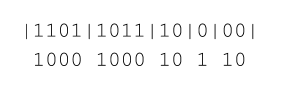
\includegraphics[width=0.4\textwidth]{images/obr_rank_select}}
\caption[Rank select usage in representation of sequence of elements with different size]{Rank/select usage for metadata. In this structure we represent elements encoded in binary as $1101_2$, $1011_2$, $10_2$, $0_2$, $00_2$.}
\label{obr:obr_rank_select}
\end{figure}

\section{Rank and select on larger alphabets}

The bit-vector data structure can be in fact used also for $\sigma = |\Sigma|>2$. One way to do this is to use one bit-vector for every possible character from $\Sigma$. This can easily use implementation of bit-vector for obtaining also working rank and select for general alphabet with the factor $\sigma$. A better way to do this is, however, using a data structure called wavelet tree described in \cite{grossi2003high} using only factor of $log\,\sigma$.

\section{Dynamic succinct data structures}

The most recent results in succinct data structures focus on how to make these data structures more usable in real-life scenarios. Many times, the
strongest assumption of these data structures is, that the data we store is not changing in any way. For a few years now, there is a considerable effort put into dynamic succinct data structures. There are different interpretations of what the word dynamic means. Let's say that our data structure represents some sequence of numbers. In some cases, it can refer to the ability to change some value in the underlying sequence. In other cases, it refers to the possibility to insert a new element at the arbitrary position in the sequence. Sometimes, it only means changing the element at an arbitrary position and adding the new element at the end of the sequence. Some dynamic data structures also allow deletion of an element.

\cite{beame2002optimal} prooved that the lower bound for dynamic rank and select is $\Omega(lg\,n/lg\,w)$. \cite{munro2015compressed} is the most recent culmination of many results in the theory of dynamic succinct data structures regarding data structures maintaining a sequence of characters from alphabet $\Sigma$. Their result obtains memory usage $nH_k+o(n\,log\,\sigma)$. Their data structure enables access, rank and select in $O(log\,n/log log\,n)$ which is optimal. Also, there is possibility to insert and delete any element in time $O(log\,n/log log\,n)$. Their solution is based on some pre-existing results and casework based on the size of $\Sigma$. This work is theoretically very strong result but contains a lot of patterns that make it not very usable and too complex in practice. It also lacks any implementation to the best of our knowledge. The insertion at an arbitrary position is many times a very strong operation that is not needed and almost always leads to a usage of a linked list that has not good memory patterns as the nodes are many times not close to each other. This all makes it not the best candidate for implementation.

\subsection{Searchable Partial Sums with Inserts Problem}

We will now introduce another type of problem that is common in relation to succinct data structures.

\begin{definition}
The Searchable Partial Sums with Inserts (SPSI) problem is asking for the data structure to
store sequence $x_1, x_2, \ldots , x_n$ of non-negative $l$-bits integers and supporting the opperations:
\begin{itemize}
    \item $sum(i) = \Sigma_{j=1}^{i} x_j$
    \item $search(s) = min(\{i; i\in \{1, 2,\ldots, n\}, \Sigma_{j=1}^{i} x_j > s \})$
    \item $update(i, k): \forall k \in Z, k \geq 0 \lor (k\leq 0 \implies x_i + k \geq 0): x_i \rightarrow x_i + k$
    \item $insert(i): x_1, x_2,\ldots, x_n \rightarrow x_1, x_2,\ldots , x_{i-1}, 0, x_{i}, \ldots , x_n$
\end{itemize}
\end{definition}

This problem is closely related to the bit-vectors and operations rank/select over them. When using the run length encoding, rank/select operations can be answered using the operations sum/search on the alternative representation of bit-vector consisting of the numbers representing lengths of runs. As can be seen in \cite{prezza2017framework}, the data structure implementing SPSI problem can be used to represent the bit-vector with rank/select operations.

\section{Existing implementations}

In this work, we focus on transforming some of the ideas that were developed over years to real implementations. Many times, the solutions aiming at the best theoretical bounds are very complicated and build on top of several ideas from previous works. Many of the current best results from the perspective of theoretical complexity do not provide any implementation. We looked at what is the current status of working implementations and what theoretical bounds they reach.

Libraries implementing succinct data structures are numerous and pretty common by now such as sdsl\cite{gog2014theory}, pizza\&chilli\cite{pizza-chilli}, libcsd\cite{brisaboa2011compressed}, succinct\cite{succinct}, sux\cite{sux}. pizza\&chilli is a framework that additionally contains a lot of tests and testing benchmarks. sdsl is one of the best libraries in terms of performance and usability. It is also very well documented. It uses the succinct representation of bit-vector and uses wavelet tree for the higher size of $\Sigma$. To the best of our knowledge, most of these frameworks only guarantee succinct representation. The main metric of these frameworks is most of the time number of bits stored as metadata as a percentage of the original data.

When we add the requirement of dynamism, we see that the number of libraries drops significantly. The most notable library supporting 
dynamic succinct data structures is DYNAMIC\cite{prezza2017framework}. It builds on top of the data structure implementing SPSI problem. Their solution uses B-tree to implement the SPSI data structure. B-tree is a type of a $(a, b)$-tree, so we are free to choose the degree of a node in the tree and also the number of elements stored in one node. Using these two parameters, we can balance the implementation to get a good tree depth and also ideal length of one node so it fits exactly into one cache line, making the implementation fast and memory friendly. Additionally, using the B-tree as an implementation for SPSI, DYNAMIC implements other succinct
data structures using their SPSI implementation such as BWT or FM-index. One of the main issues of DYNAMIC implementation is bad cooperation of their solution with the default allocator which hampers the memory usage due to the high memory fragmentation.

Idea of dynamic bit-vector from \cite{policriti2015average} can be found implemented in \cite{ds-bitvector}. This bit-vector supports insertions at an arbitrary position using the succinct representation. It is also implemented as a packed B-tree.

The other two notable and recent results that both dominate DYNAMIC in terms of speed and extra space usage are \cite{marchini2020compact} and \cite{pibiri2020rank}.

Marchini et al. got better results than DYNAMIC using a compressed Fenwick tree\cite{marchini2020compact}, the data structure used for logarithmic prefix sum queries and updates\cite{fenwick1994new}. The structure of the Fenwick tree is further changed so that it fits nicely with good memory access patterns. The most recent solution, solving the same problem as is described by Marchini is described in \cite{pibiri2020rank} by Pibiri et al. Their implementation is tailored for modern processors, using parallel SIMD instructions. Performance of their solution can be even compared with most of the static data structures. Similarly, as a Marchini et al., they interpret the problem as a dynamic prefix sum problem with the difference of using a segment tree instead of a Fenwick tree.

\section{Proposed solution}

Our main objective is to build dynamic data structure, representing the sequence of elements with the operations access, rank, select and dynamic operations replace, insert/delete with the guaranteed memory usage at most $nH_k+o(n\lg\sigma)$ which corresponds to high-order compressed representation. We want to achieve also the best possible time complexity for $rank$ and $select$ but we do not target any specific time complexity class as we want to make our implementation as fast as possible on the current computer model. The only requirement for our operations is to have time complexity at most $O(\log n)$. Our first step towards our goal is to create a data structure for binary alphabet. We think that this will be easier as the usage of special CPU instructions will be more straightforward. Then we would like to take some of the ideas and our experience to develop also the general solution for any meaningful size of $\Sigma$. For a few years, there was an effort in this field to match lower bounds that were proven for the dynamic succinct data structures. Now, we think that there is a significant gap between the real implementations and the ones that achieve theoretical lower bounds. We also think that it will be theoretically challenging to relax some of the time complexities in order to maintain fast and usable implementation with still guaranteed high-order compressed representation.
